\documentclass[twoside]{article}
\setlength{\oddsidemargin}{0.25 in}
\setlength{\evensidemargin}{-0.25 in}
\setlength{\topmargin}{-0.6 in}
\setlength{\textwidth}{6.5 in}
\setlength{\textheight}{8.5 in}
\setlength{\headsep}{0.75 in}
\setlength{\parindent}{0 in}
\setlength{\parskip}{0.1 in}

\usepackage{graphicx}
\usepackage{url}

%
% The following commands sets up the lecnum (lecture number)
% counter and make various numbering schemes work relative
% to the lecture number.
%
\newcounter{lecnum}
\renewcommand{\thepage}{\thelecnum-\arabic{page}}
\renewcommand{\thesection}{\thelecnum.\arabic{section}}
\renewcommand{\theequation}{\thelecnum.\arabic{equation}}
\renewcommand{\thefigure}{\thelecnum.\arabic{figure}}
\renewcommand{\thetable}{\thelecnum.\arabic{table}}
\newcommand{\dnl}{\mbox{}\par}

%
% The following macro is used to generate the header.
%
\newcommand{\lecture}[4]{
  \pagestyle{myheadings}
  \thispagestyle{plain}
  \newpage
  \setcounter{lecnum}{#1}
  \setcounter{page}{1}
  \noindent
  \begin{center}
  \framebox{
     \vbox{\vspace{2mm}
   \hbox to 6.28in { {\bf COMPSCI~590S~~~Systems for Data Science
                       \hfill Fall 2016} }
      \vspace{4mm}
      \hbox to 6.28in { {\Large \hfill Lecture #1: #2  \hfill} }
      \vspace{2mm}
      \hbox to 6.28in { {\it Lecturer: #3 \hfill Scribe(s): #4} }
     \vspace{2mm}}
  }
  \end{center}
  \markboth{Lecture {#1}: #2}{Lecture {#1}: #2}
  \vspace*{4mm}
}

%
% Convention for citations is authors' initials followed by the year.
% For example, to cite a paper by Leighton and Maggs you would type
% \cite{LM89}, and to cite a paper by Strassen you would type \cite{S69}.
% (To avoid bibliography problems, for now we redefine the \cite command.)
%
\renewcommand{\cite}[1]{[#1]}

% \input{epsf}

%Use this command for a figure; it puts a figure in wherever you want it.
%usage: \fig{NUMBER}{FIGURE-SIZE}{CAPTION}{FILENAME}
\newcommand{\fig}[4]{
           \vspace{0.2 in}
           \setlength{\epsfxsize}{#2}
           \centerline{\epsfbox{#4}}
           \begin{center}
           Figure \thelecnum.#1:~#3
           \end{center}
   }

% Use these for theorems, lemmas, proofs, etc.
\newtheorem{theorem}{Theorem}[lecnum]
\newtheorem{lemma}[theorem]{Lemma}
\newtheorem{proposition}[theorem]{Proposition}
\newtheorem{claim}[theorem]{Claim}
\newtheorem{corollary}[theorem]{Corollary}
\newtheorem{definition}[theorem]{Definition}
\newenvironment{proof}{{\bf Proof:}}{\hfill\rule{2mm}{2mm}}

% Some useful equation alignment commands, borrowed from TeX
\makeatletter
\def\eqalign#1{\,\vcenter{\openup\jot\m@th
 \ialign{\strut\hfil$\displaystyle{##}$&$\displaystyle{{}##}$\hfil
     \crcr#1\crcr}}\,}
\def\eqalignno#1{\displ@y \tabskip\@centering
 \halign to\displaywidth{\hfil$\displaystyle{##}$\tabskip\z@skip
   &$\displaystyle{{}##}$\hfil\tabskip\@centering
   &\llap{$##$}\tabskip\z@skip\crcr
   #1\crcr}}
\def\leqalignno#1{\displ@y \tabskip\@centering
 \halign to\displaywidth{\hfil$\displaystyle{##}$\tabskip\z@skip
   &$\displaystyle{{}##}$\hfil\tabskip\@centering
   &\kern-\displaywidth\rlap{$##$}\tabskip\displaywidth\crcr
   #1\crcr}}
\makeatother

% **** IF YOU WANT TO DEFINE ADDITIONAL MACROS FOR YOURSELF, PUT THEM HERE:



% Some general latex examples and examples making use of the
% macros follow.

\begin{document}

%FILL IN THE RIGHT INFO.
%\lecture{**LECTURE-NUMBER**}{**DATE**}{**LECTURER**}{**SCRIBE**}
\lecture{17}{Latency-Tolerant Software Distributed Shared Memory}{Emery
  Berger}{Jun Wang, Abhinav Tushar}
  
In this lecture we discussed Grappa, a distributed shared memory system and more
generally, touched the differences between a shared memory (like Grappa) and a
distributed memory system (like MapReduce).

\section{Shared Memory vs. Distributed Memory Systems}

A shared memory system works with a global addressing space for all the machines
while a distributed memory system works with machine local addressing. Having
different address spaces in distributed memory can result in issues due to
concurrency.

Explicit message passing, instead of using memory read/write abstraction, can
result in non deterministic message delivery. Moreover, concurrency due to
multiple cores of a single machine is another source of uncertainty. These can
result in data races and inconsistent world views for each of the machines. Debugging
these distributed memory systems is also a problem. A debugger relies on a
consistent global view to provide the following features:

\begin{itemize}
\item Breakpoints
\item Watchers
\item Stepping
\item Memory inspection and manipulation
\end{itemize}

In a distributed system, there are multiple stacks, heaps and threads to keep
track of and due to lack of a global view at any machine, it becomes hard to
find and ascribe bugs.

\section{Addressing in shared memory systems}

Addressing in shared memory systems involves converting memory access
instructions to network messages. For example if a program asks for the value of
a variable $x$ (say), the system has to figure out if the variable is mapped to
current machine or is somewhere else. In first case, it will be a simple memory
read. In second, it has to be a network message that fetches the data from a
remote machine.

A global addressing space can be provided by either of these:

\begin{itemize}
\item Compiling the program in a way that considers the data partition among the
  machines and substitutes message passing for direct reads / writes whenever
  needed.
\item Create a library which provides global classes which inherently are made
  to work with partitions.
\end{itemize}


In any case, there are performance issues due to locality. These are usually
addressed by either:
\begin{itemize}
\item {\sl Partitioning} the data among machines.
\item {\sl Prefetching}. A fetch-on-need scheme is costly as it exposes the
  network latency in the main program sequence. Aggregating small network
  messages, can hide the network latency under bandwidth.
\item {\sl Make it parallel}. Parallelizing the code is another way to hide
  latency. In a highly parallelized system, many pending network messages will
  not hurt that much because there will always be sufficient number of threads
  busy in actual computation, while the network latency involving other threads
  gets hidden.
\end{itemize}
\section{Insights of the Grappa system}
\begin{enumerate}
\item {\bf New workloads}\\
The workload of big data matches the good case of the shared memory. Rather than
a single thread program randomly accesses memory, we have a lot of processor
processing working over big data in embarrassingly parallel.
\item {\bf New technologies}
\begin{itemize}
\item {\sl InfiniBand}\\
InfiniBand is a  an architecture and specification which features low latency
high bandwidth It is widely used in high end servers.
\item {\sl RDMA}\\
RDMA, Remote Direct Memory Access, is a direct memory access from the memory of
one computer into that of another without through either one's kernel. It
provides high-throughput and low-latency.
\end{itemize}
\end{enumerate}

\section{Message Ordering}
How to order events (e.g. messages) in distributed system? Events are naturally
ordered in a single processor machine. But in a distributed system without
global clock, local clocks may be unsynchronized and therefore events cannot be
ordered by local times.
However, our interest is not on obtaining and maintaining true time, but on
getting event sequence that be agreed system-wide. To achieve this goal,
``happened before'' relation is developed: $a\rightarrow b$ means that $a$
happens before $b$. If $a$ is a message send and $b$ is message being received,
then $a\rightarrow b$ must be true.
Lamport clock and vector clock are two algorithms using ``happened before''
relation.
\subsection{Lamport clock}
Lamport's algorithm:
\begin{itemize}
\item Each message carries a timestamp of the sending time according to sender's
  clock;
\item When a message arrives and the receiver's clock is less than the timestamp
  on the received message, the system’s clock is forwarded to the message's
  timestamp + 1. Otherwise, the message is recognized as out of order and
  nothing is done.
\end{itemize}
An example is shown in Figure \thelecnum.1.
\begin{figure}[h]
\centering
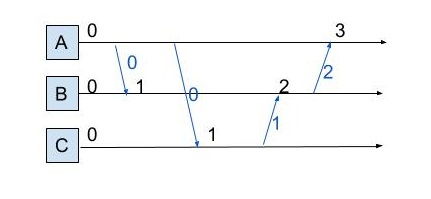
\includegraphics[width=0.7\linewidth]{lamport}
\caption[]{Example of Lamport clock}
\label{cpl}
\end{figure}

\subsection{Vector clock}
Vector clock is a generalization of Lamport clock. A vector clock in a system of
N processes is a vector of N integers. Each process maintains its own vector
clock to timestamp local events. Like Lamport timestamps, vector timestamps (the
vector of N integers) are sent with each message.

\end{document}
